\documentclass[11pt,a4paper]{article}
\usepackage[T1]{fontenc}
\usepackage{lmodern}
\usepackage{microtype}
\usepackage[margin=25mm]{geometry}
\usepackage{amsmath,amssymb}
\usepackage{graphicx}
\usepackage{booktabs}
\usepackage[font=small,labelfont=bf]{caption}
\usepackage[dvipsnames]{xcolor}
\usepackage[hidelinks]{hyperref}
\ifdefined\pdftrailerid\pdftrailerid{}\fi

% A result that does not exist yet is shown as a visible placeholder, never as a value (plan P1).
\newcommand{\pending}[1]{\textcolor{BrickRed}{[pending: #1]}}
\input{generated/numbers.tex}

\title{Did UK recessions give warning?\\[2pt]\large A preregistered test of rising AR(2) persistence before recession onsets}
\author{Kostadin Stoyanov}
\date{Draft, \notedate}

\begin{document}
\maketitle

\begin{abstract}
\noindent Before UK recessions since 1955, did the economy's memory---the largest modulus $M(t)$ of the roots of a rolling second-order autoregression fitted to quarterly real GDP growth---rise towards the unit circle more than constant dynamics would produce by chance? The sample, statistic, surrogate null, decision rule and random streams were registered before the data were acquired (OSF, \href{https://doi.org/\DOI}{doi:\DOI}). \HoneConclusion{} As a check on the method's oldest ancestor, Yule's (1927) sunspot equation is reproduced from his own printed data and compared across two versions of the sunspot series.
\end{abstract}

\section{Question}

Let $g_t$ be annualised quarterly growth of UK real GDP and fit, in each window of $W=40$ quarters ending at $t$, the regression $g_s = c + \varphi_1 g_{s-1} + \varphi_2 g_{s-2} + \varepsilon_s$. The largest root modulus $M(t)=\max(|\lambda_1|,|\lambda_2|)$ of $\lambda^2-\varphi_1\lambda-\varphi_2=0$ measures persistence: $M$ near one means shocks die out slowly. For each recession onset $r$ the change $\Delta_r = M(r-1)-M(r-9)$ compares the eight quarters before the onset with the window ending two years earlier. The primary hypothesis H1 is one-sided: the mean change $S$ over eligible recessions is larger than a fitted constant-parameter AR(2) would produce by chance.

\section{Background}

Yule (1927) introduced the second-order autoregression to describe sunspot numbers as a ``disturbed'' oscillation: a damped harmonic motion kept alive by random impulses. His equation for Wolfer's numbers, 1749--1924, was $u_x = \YuleBone\,u_{x-1} - \YuleBtwo\,u_{x-2} + \YuleConst$, with a period of \YulePeriod{} years. The same object---two roots inside the unit circle, with persistence measured by their modulus---is the indicator studied here.

Critical slowing down predicts that a system losing resilience as it approaches a transition recovers more slowly from small shocks, so that autocorrelation rises beforehand (Scheffer et al., 2009; Dakos et al., 2012). Tests on financial data have found weak or mixed evidence (Guttal et al., 2016; Diks et al., 2019). The nearest macroeconomic work is Rye and Jackson (2020), whose abstract and methods describe lag-one autocorrelation and variance computed on historical GDP datasets, with attention to variability over several decades. H1 instead specifies recession-onset contrasts in the fitted root modulus, an endogenous-onset surrogate comparison and a protocol registered before the present data analysis. This distinction is not a claim of established novelty.

\section{Data}

\textbf{UK output.} ONS series ABMI (gross domestic product, chained volume measures, seasonally adjusted), quarterly levels 1955Q1--2019Q4, from the latest quarterly national accounts publication released before the registration was approved. The release rule was registered in advance; the release identity, file hash and retrieval time are recorded in \texttt{DATA\_MANIFEST.csv}. \ReleaseIdentity{} Growth is $g_t = 400\,(\ln Y_t - \ln Y_{t-1})$, 259 observations, 1955Q2--2019Q4. Onsets from 2020 onwards are outside the test.

\textbf{Sunspots.} SILSO yearly mean total sunspot number, Version~1.0 (frozen archive, 1700--2014) and Version~2.0 (1700--2025, retrieved 27 September 2026), and Wolfer's numbers for 1749--1924 as printed in Yule's Table~A, transcribed with page references and checked against Yule's own printed arithmetic. All files and hashes are listed in the data manifest.

\section{Method}

Every rule below was fixed in the registered protocol before the UK data were acquired; the protocol is the authoritative text.

\begin{enumerate}\itemsep2pt
\item \textbf{Rolling fits.} Each window of $W=40$ growth observations is fitted on its own by least squares with an intercept, its first two values serving only as lags. Coefficients are not constrained; $M(t)$ is not clipped.
\item \textbf{Recessions.} A qualifying run is two or more consecutive quarters of negative growth, with onset its first quarter. A run beginning within eight quarters of the previous run's end joins that episode; only the episode's first onset counts. An onset is eligible if $M(r-9)$ exists.
\item \textbf{Statistic.} $S$ is the mean of $\Delta_r$ over the $m$ eligible episodes; all signs are kept and $k=\#\{\Delta_r>0\}$ is reported.
\item \textbf{Null.} One AR(2) is fitted to the whole sample and must be strictly stable. Each of $B=1{,}000$ surrogates resamples its centred residuals with replacement and rebuilds a series of length 259 from the first two observed values. Every surrogate is analysed exactly as the data, including detecting its own recessions; surrogates with no eligible episode are dropped and counted.
\item \textbf{Decision.} $p=(1+\#\{S_b\ge S\})/(B'+1)$ over the $B'$ retained surrogates; the specified comparison rejects when $p\le 0.05$. A valid $p>0.05$ is reported as inconclusive. A retained diagnostic compares the upper end of a 90\% episode-resampling interval for $S$ with the detectable change $D_{80}$ from the power study; it does not establish absence.
\item \textbf{Secondary analyses}, all reported: windows of 32 and 48 quarters; surrogates evaluated at the observed onset dates; wild-bootstrap signs; the Kendall trend of $M$ over the 16 quarters before each onset; and lag-one autocorrelation in the same windows.
\item \textbf{Validation before data.} White-noise complex-root rates at lengths 30 and 1,000 (AT-5), the size of the test on 200 constant-parameter series (AT-15), and power over four planted-signal strengths (AT-16) were run under the registered design before acquisition. Random numbers come from PCG64 generators with registered stream identifiers and master seed 1927.
\end{enumerate}

\noindent Registration: \href{https://doi.org/\DOI}{doi:\DOI}, submitted on \RegistrationSubmitted{} and approved at \RegistrationApproved{}.
Validation: G2 \GtwoStatus; AT-5 complex-root rates \ATfiveThirty{} ($n=30$) and \ATfiveThousand{} ($n=1{,}000$); AT-15 rejection rate \ATfifteen; $D_{80}=\,$\Deighty.

\section{Results}

\subsection{H1}

The primary statistic is $S=\,$\HoneS{} over $m=\,$\HoneM{} eligible recessions, $k=\,$\HoneK{} of them positive, with $p=\,$\HoneP{} from $B'=\,$\HoneRetained{} retained surrogates (Figure~\ref{fig:h1}). \HoneConclusion{} The 90\% episode-resampling interval for $S$ is \HoneInterval, a conditional diagnostic without asserted coverage. \HoneBranchB

\begin{figure}[htbp]
\centering
\IfFileExists{../figures/h1_persistence.pdf}{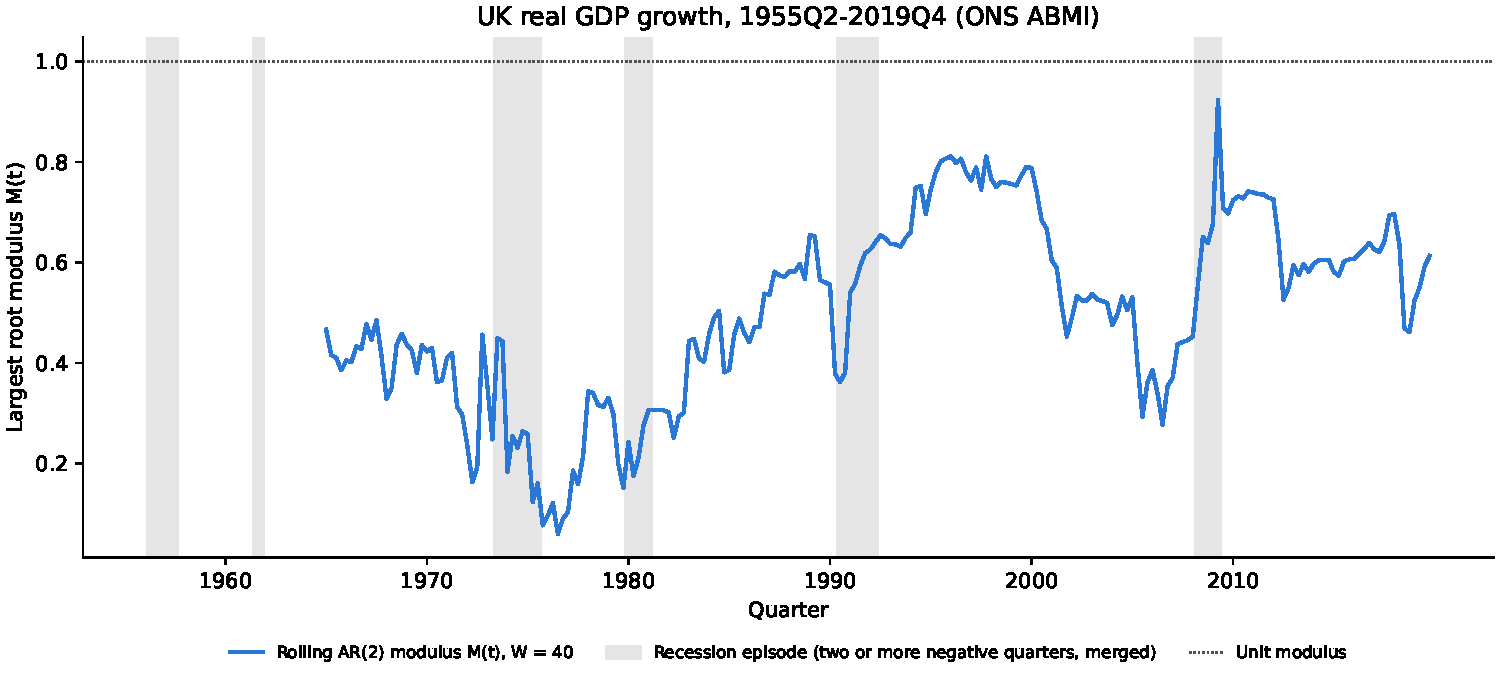
\includegraphics[width=\linewidth]{../figures/h1_persistence.pdf}}{\pending{figure: the $M(t)$ path with recessions shaded, after the registered run}}
\caption{Rolling AR(2) modulus $M(t)$, $W=40$, with recession episodes shaded.}
\label{fig:h1}
\end{figure}

\input{generated/h1_tables.tex}

\subsection{S1: the Yule centenary}

Rounding the deviations of Wolfer's numbers from their mean to the nearest unit, as Yule describes, reproduces his serial correlations exactly ($r_1=\YuleRone$, $r_2=\YuleRtwo$) and his equation to within $10^{-5}$ (Table~\ref{tab:s1}). On the same numbers the programme's least-squares estimator gives a period of \TableALSPeriod{} years and its Yule--Walker convention \TableAYWPeriod{} years, against Yule's \YulePeriod: his figure reflects his correlation arithmetic rather than his data. His printed numbers differ from SILSO's frozen Version~1 in \TableADiffVone{} of 176 years, by at most \TableAMaxDiff.

The 2015 recalibration changes little. For 1749--1924, Version~2 lengthens the least-squares period from \VoneLSPeriod{} to \VtwoLSPeriod{} years (a shift of \PeriodShift) and moves the modulus from \VoneLSModulus{} to \VtwoLSModulus; the bootstrap band for the Version~1 period runs from \VoneLSBandLow{} to \VoneLSBandHigh{} years (Figure~\ref{fig:s1}). Bands and point differences are reported; no difference test was registered.

\begin{table}[htbp]
\centering\small\setlength{\tabcolsep}{4.5pt}
\input{generated/s1_table.tex}
\caption{Yule's sunspot AR(2): as printed, reproduced from his Table~A, and refitted on SILSO Versions~1 and~2. Bands are 95\% percentile intervals for the period from 4,000 residual-bootstrap draws.}
\label{tab:s1}
\end{table}

\begin{figure}[htbp]
\centering
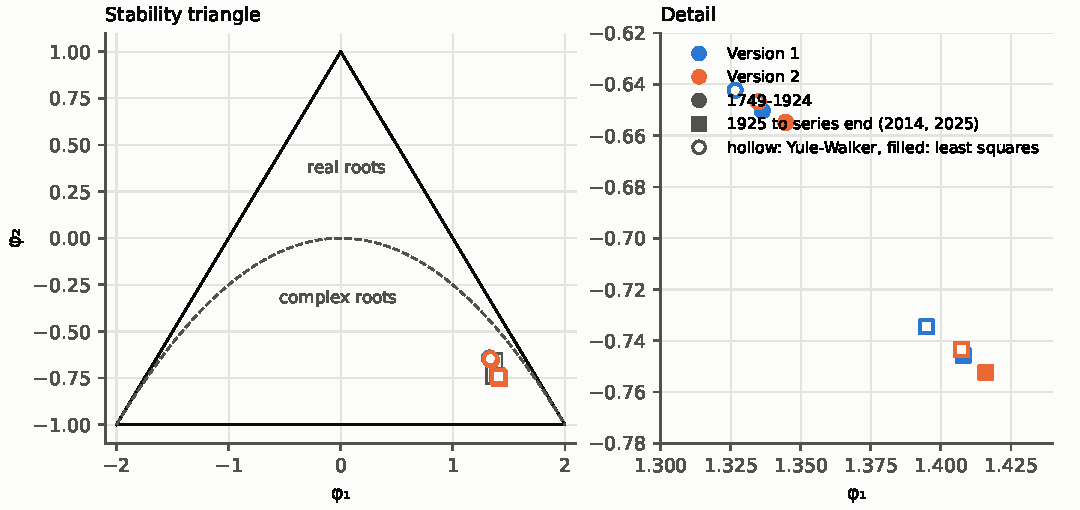
\includegraphics[width=0.92\linewidth]{../figures/s1_triangle.pdf}
\caption{The sunspot fits in the stability triangle; the dashed curve separates real from complex roots.}
\label{fig:s1}
\end{figure}

\subsection{S2: the Samuelson reading, a check}

Samuelson's (1939) multiplier--accelerator model implies a second-order autoregression in output, so a fitted AR(2) can be read back as a multiplier $c=\varphi_1+\varphi_2$ and an accelerator $v=-\varphi_2/(\varphi_1+\varphi_2)$, oscillating when $c>0$ and $c(1+v)^2<4v$. The reading depends on how the cycle is separated from trend. Three filters were fixed before the data: a linear trend, the Hodrick--Prescott filter with $\lambda=1600$, and Hamilton's (2018) regression filter with $h=8$ and $p=4$. This is standard teaching material, reported as a check and not as a result.

\input{generated/s2_body.tex}

\section{Limitations}

Few recessions enter the test and their windows overlap, so the episode interval is coarse and has no established coverage. The null is a fitted constant-parameter AR(2): rejecting it does not show a positive rise in persistence, and not rejecting it does not show its absence. Recessions are selected from the same series that is tested, which the surrogates reproduce only under the null. The result is conditional on one data vintage, a two-quarter recession rule and a 40-quarter window; the secondary analyses show how much each choice matters. Nothing here concerns causal tipping, individual recessions or real-time forecasting.

\section{An error in this work}

The first Kalman filter written for the programme's state-space foundations failed its own acceptance test: with a diffuse prior of $10^8$ its final state differed from least squares by \ATelevenFirst, against a target of $10^{-6}$. The cause was rounding in the covariance recursion, which subtracts numbers of order $10^8$ to obtain entries of order $10^{-4}$. The failure was published before the fix; a square-root form now agrees to \ATelevenFixed, the exact-arithmetic value.

\section{The next question}

A white-noise series of length 30 shows complex roots---an apparent cycle---in \ATfiveThirtyPercent{} of least-squares AR(2) fits (AT-5). When does a fitted AR(2) imply a cycle that is really there, and what test of it has the right error rate?

\section*{Reproducibility}

Code, data manifest, registered protocol and every evidence record are in the \texttt{unit-circle} repository. Each number in this note is written from those records by \texttt{tools/build\_note.py}; \texttt{make note} rebuilds the note, and the other \texttt{make} targets rebuild each record and figure from the raw files.

\section*{References}
\small
\begin{description}\itemsep0pt
\item Dakos, V. et al. (2012) Methods for detecting early warnings of critical transitions in time series illustrated using simulated ecological data. \emph{PLoS ONE} 7(7), e41010.
\item Diks, C., Hommes, C. and Wang, J. (2019) Critical slowing down as an early warning signal for financial crises? \emph{Empirical Economics} 57(4), 1201--1228.
\item Guttal, V. et al. (2016) Lack of critical slowing down suggests that financial meltdowns are not critical transitions, yet rising variability could signal systemic risk. \emph{PLoS ONE} 11(1), e0144198.
\item Hamilton, J. D. (2018) Why you should never use the Hodrick-Prescott filter. \emph{Review of Economics and Statistics} 100(5), 831--843.
\item Rye, C. D. and Jackson, T. (2020) Using critical slowing down indicators to understand economic growth rate variability and secular stagnation. \emph{Scientific Reports} 10, 10481.
\item Samuelson, P. A. (1939) Interactions between the multiplier analysis and the principle of acceleration. \emph{Review of Economic Statistics} 21(2), 75--78.
\item Scheffer, M. et al. (2009) Early-warning signals for critical transitions. \emph{Nature} 461, 53--59.
\item Yule, G. U. (1927) On a method of investigating periodicities in disturbed series, with special reference to Wolfer's sunspot numbers. \emph{Philosophical Transactions of the Royal Society A} 226, 267--298.
\end{description}

\end{document}
